\documentclass[]{article}
\usepackage{hyperref}
\usepackage{amsmath}
\usepackage[utf8]{inputenc}
\usepackage[parfill]{parskip}
%\usepackage[english]{babel}
\usepackage[autostyle]{csquotes}
%\usepackage[style=numeric,backend=biber]{biblatex}
\usepackage[pdftex]{graphicx} % Image import.
\usepackage{pgfplots}
\usepackage{float}

%\addbibresource{biblio.bib}

\newcommand{\clique}{\textsc{clique}}
\newcommand{\sat}{\textsc{sat}}

%opening
\title{Approaching the Clique Problem\\ With SAT Solvers\\[.2cm]
	\large{CIS 673: Computer Aided Verification}}
\author{Matthew Howard}

\begin{document}
	
	\maketitle
	
	\begin{abstract}
		Modern SAT solvers are able to solve real world instances of \textsc{sat} within realistic time and space restrictions. General purpose solvers have been effective in solving artificial intelligence problems, circuit design, logic puzzles, and verification problems. For this project, we evaluate the application of a SAT solver to the classical graph theoretic \clique{} problem.
	\end{abstract}
	
	\section{Introduction}
	
	
	\section{The Clique Problem}
	
	Let us start by defining terminology. A \textit{graph} is a duple $G = (V, E)$ consisting of a vertex set $V$ and an edge set $E \subseteq \{(u, v) ~\vert~ u, v \in~V, u \neq v\}$. We will also follow the convention $n = |V|$ and $m = |E|$. An \textit{induced subgraph} $G' = (V', E')$ of $G$ consists of a vertex set $V' \subseteq V$ and the maximal edge subset $E' \subseteq E$ such that the endpoints of each edge are in $V'$, formally $E' = \{(u, v) \in E ~\vert~ u, v \in V'\}$. For the purpose of this report, we are concerned only with undirected, unweighted graphs.
	
	A graph is \textit{complete} if there exists an edge between any two distinct vertices.
	
	A \textit{clique} $G' = (V', E')$ in $G$ is an induced subgraph which is also a complete graph. We say a clique is of size $k$ if its vertex set contains $k$ elements. The \textit{Clique Problem}, which we refer to as \clique{}, given a graph $G$ and a positive integer $k$, is the problem of determining whether there exists an induced subgraph $G'$ satisfying the following two conditions:
	\begin{enumerate}
		\item \textbf{(Clique Condition)} $G'$ is a clique in $G$
		\item \textbf{(Size Condition)} $G'$ is of size at least $k$
	\end{enumerate}	
	
	Notice that for a clique $G'$ in $G$, every induced subgraph $G''$ of $G'$ is also a clique in $G$, so we could equivalently formulate \clique{} with a more strict size property ``$G'$ is of size exactly $k$''.
	
	While we are concerned mostly with the decision problem formulation of \clique{}, it's worth drawing attention to the optimization formulation: Given a graph $G'$, find a clique of maximum size. We call refer to the maximum clique size of a graph $\omega(G)$. The optimization and decision versions are similar in complexity. If $\omega(G)$ is known, then the decision problem is equivalent to checking if $k \le \omega(G)$. Likewise, if we have an oracle for \clique{} which provides the clique's vertex set as a certificate, then we can solve the optimization version in $O(\log n)$ calls to the oracle using a binary search of $k$.
	
	The clique problem is of significance is complexity theory for a few reasons. It is one of the classical NP-complete problems. It is in NP since the vertex set of a $k$ clique can serve as a $O(n)$ certificate from which it is easy to verify the Clique and Size properties. The problem can be shown to be NP-hard through the two reductions
	\begin{align}
	\textsc{sat} \le_p \textsc{3sat} \le_p \clique
	\end{align}
	
	Second, the hardness of \clique{} is often exploited in proving the NP-hardness of \textsc{vertex-cover} and other NP-hard problems which indicates its usefulness in constructing reduction proofs. Finally, \clique{} is ``hard'' in the algorithmic sense that there does not exist an approximation algorithm which performs better than $n^{1 - \epsilon}$\cite{Hastad1999}.
	
	\section{SAT Solvers}
	Rather than performing a survey of different SAT solvers (which is done each year in the SAT competition), we chose to focus our efforts one solver in particular. We decided to go with MiniSat because it is widely used, open source, minimalistic, and designed for integration. MiniSat is based on conflict-driven learning and unit propagation and is implemented in C++.\cite{Een03anextensible}
	
	%TODO Where do we put this?
	%\section{Other Graph Metrics}
	
	\section{Obtaining Data Sets}
	We want to analyze our clique solver on both real-world and randomly-generated graphs. We originally intended to collect data from the Facebook friend network of the author. For instance, vertices would correspond to friends of the author (not including the author as a vertex) and edges would correspond to friendships between vertices in the graph. Running analyses on real data allows us to draw social insights from the resulting cluster. For example, it would be interesting to identify common traits between the people composing the largest clique, e.g. membership in a club.
	
	\subsection{Social Network Data}
	The Facebook Graph API provides REST access to the required information, including lists of friends and lists of mutual friends in easily parsable formats. However, since the release of version 2.0 of the API, lists will only show friends who have actively logged into the API Application (in this case our data collection tool)\footnote{\url{https://developers.facebook.com/bugs/1502515636638396/}}. This severely restricts the usefulness of this data. One alternative to collecting the same data would be to write a web-scraping tool using a browser automation tool like Selenium. However, this solution begs difficult ethical and legal implications since neither Facebook nor the users consent to this style of data collection.
	
	Luckily, the Stanford Network Analysis Project provides a number of anonymized, real-world datasets including a 4039-node graph of Facebook friend data. While the anonymous nature of this data limits social insights that could come out of our analysis, the data will nonetheless fulfill our goal of testing our solvers on real-world data.
	
	The Stanford Datasets provides us with ten graphs of varying sizes. We label these graphs \texttt{facebook.a} through \texttt{facebook.j}.
	
	\subsection{Random Datasets}
	Since the Facebook datasets are limited in number and cannot be generated to be arbitrary large, we want another source of graph data. We wrote a script to generate a Erdős - Renyi graph (i.e. edges chosen uniformly at random) given values for $n$ and $m$. Then, we generated ten graphs with values of $n$ and $m$ matching those of the Facebook graphs. We label these \texttt{random.a} through \texttt{random.j}.
	
	\subsection{Analyzing the Data}
	Before we run and evaluate our clique solver, we want to analyze the graph datasets. We leverage ``igraph'', a graph analysis library with a Python wrapper to collect the following statistics:
	\begin{enumerate}
		\item $n$ and $m$, the number of nodes and edges in the graph
		\item Edge density, defined as $\frac{m}{n (n - 1) / 2}$
		\item Diameter, the maximum eccentricity of nodes in $G$
		\item Radius, the minimum eccentricity of nodes in $G$
		\item Number of connected components
		\item $\omega(G)$, as well as the time required to compute $\omega(G)$
	\end{enumerate}
	where the eccentricity of a vertex $v$ is $\epsilon(v) = \max_{u \in V} distance(u, v)$.
	
	igraph's $\omega(G)$ function is based off of an algorithm due to Tsukiyama \textit{et al.} and has a worst-case runtime of $O\left(3^{n/3}\right)$. This algorithm will serve as a point of comparison for the performance of our \clique{} solver.
	
	\section{Reduction Strategy}
	Given a graph $G$ and a positive integer $k$, we want to produce an instance of \sat{}. Every \sat{} instance consists of variables and clauses. Since a clique is defined by its vertex set and a solution to \sat{} is defined by a set of variable assignments, we naturally correspond vertices to variables. For all $v \in V$, let $x_v$ represent the variable indicating whether $v \in V'$.
	 
	Now, we need some way of encoding edges. The Size Condition in \clique{} is independent of the edge set $E$ and just relies on the variables in the vertex set $V'$. Therefore, we must reference our edge set $E$ in the Clique Condition.
	
	We restate our Clique Condition as:
	\begin{align}
	\forall~u,v \in V,&& \quad u \in V' \land v \in V' &\implies (u, v) \in E \\
	\forall~u,v \in V,&& x_u \land x_v &\implies (u, v) \in E
	\end{align}
	
	If we take the contrapositive, we get
	\begin{align}
	\forall~u,v \in V,&& (u, v) \notin E &\implies \lnot x_u \lor \lnot x_v \\
	\forall~u,v \in V,&& (u, v) \in \overline{E} &\implies \lnot x_u \lor \lnot x_v\\
	\forall~ (u, v) \in \overline{E},&& &\lnot x_u \lor \lnot x_v
	\end{align}
	where $\overline{E}$ is the complement edge set, $\overline{E} = \{(u, v) ~\vert~ u, v \in~V, u \neq v\} \setminus E$. This last statement of the clique condition can easily be encoded in \sat{} since $\lnot x_u \lor \lnot x_v$ is a CNF clause, and $\overline{E}$ is an enumerable set of size $O(n^2 - m)$ over which we can add clauses.
	
	The Size Condition is a bit trickier. We need to add variables and clauses that require at least $k$ of our vertex variables be true. If we number our vertices $1 \ldots n$ and consider our vertex variables as binary indicator variables, we want
	\begin{align}
	\sum_{i = 1}^{n} x_i \ge k
	\end{align}
	The computation on the left hand side can be represented as a combinational digital circuit with $n$ single-bit inputs and one $(\lfloor\log_2 n\rfloor + 1)$-bit output. Let us define $k'$ to be the least natural number such that $k + k'$ is a power of 2, say $2^p$. Adding $k'$ to both sides, we get 
	\begin{align}
	\sum_{i = 1}^{n} x_i + k' \ge k + k'
	\end{align}
	This expression is equivalent to checking whether the $p$-th bit of the sum on the left hand size is equal to 1, which can be expressed as a one-literal clause.
	
	\begin{figure}[H]
		\caption{Adder Tree Schematic}
		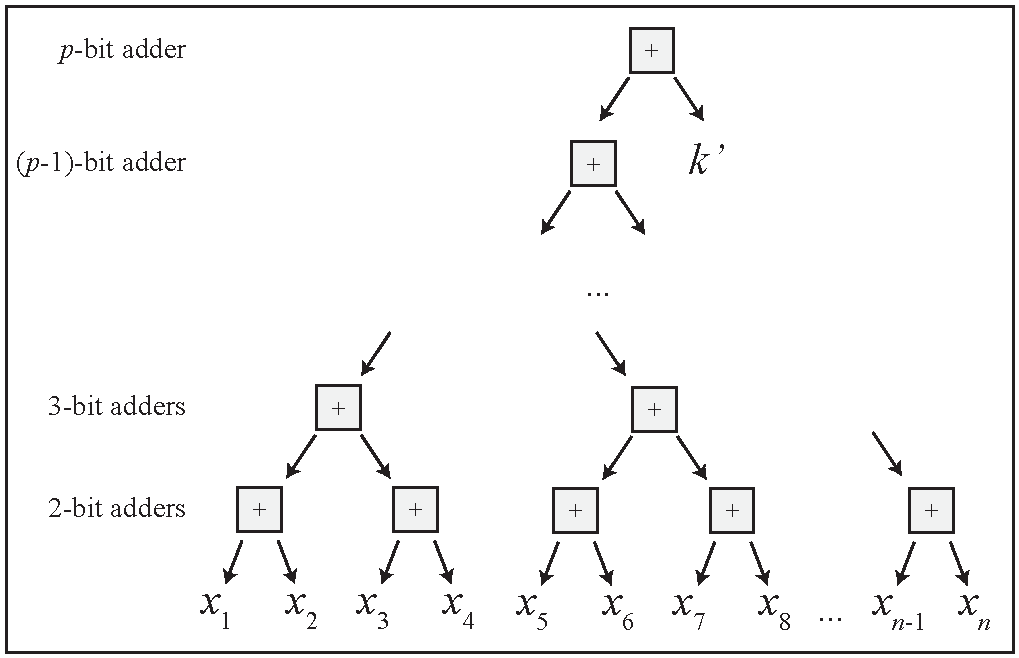
\includegraphics[width=4.5 in]{adder-tree}
		\centering
	\end{figure}
	
	We implement the sum using an adder tree. The leaves of the tree are the vertex variables and $k'$ while the internal nodes are binary adders of varying size. The $j$-bit binary adders are constructed from full adders, which are constructed from NAND and NOR gates, which are constructed from boolean clauses plus additional variables.
	\section{Evaluation}
	
	\section{Conclusion}
	
	\section{References}
	
	%\nocite{*}
	
	%\printbibliography
	
\end{document}
